\documentclass[a4paper]{article}

\usepackage{fullpage} % Package to use full page
\usepackage{parskip} % Package to tweak paragraph skipping
\usepackage{tikz} % Package for drawing
\usepackage{amsmath}
\usepackage{hyperref}
\usepackage{ctex}
\usepackage{amssymb}
\usepackage{amsthm}
\usepackage{indentfirst}
\setlength{\parindent}{2em}
\usepackage{array}
\usepackage{graphicx}
\usepackage{float} 
\usepackage{subfigure}

\renewcommand\thefigure{\thesection.\arabic{figure}}
\makeatletter
\@addtoreset{figure}{section}
\makeatother

\renewcommand\thesubfigure{\thesection.\arabic{figure}(\alph{subfigure})}
\makeatletter
\@addtoreset{figure}{section}
\makeatother

\makeatletter
\renewcommand \theequation {%
	\ifnum \c@section>\z@ \@arabic\c@section.\fi \ifnum \c@subsection>\z@
	\@arabic\c@subsection.\fi\ifnum \c@subsubsection>\z@
	\@arabic\c@subsubsection.\fi\@arabic\c@equation}
\@addtoreset{equation}{section}
\@addtoreset{equation}{subsection}
%\setcounter{section}{-1}
\makeatother

\hypersetup{
	colorlinks=true,
	linkcolor=black
}

\title{高等数值分析}
\author{罗雁天 \\
2018310742}
\date{\today}

\begin{document}

%\maketitle
\newcommand{\HRule}{\rule{\linewidth}{0.5mm}}
\begin{titlepage}
	\begin{center}
		% Upper part of the page
		
\includegraphics[width=0.4\textwidth]{Tsinghua2.png}\\[1cm]
		\textsc{\Large \texttt{高等数值分析}}\\[1cm]
		% Title
		\HRule \\[1cm]
		{\Huge \bfseries 病态线性方程组的求解}\\[0.4cm]
		\HRule \\[3.5cm]
		% Author and supervisor
		\begin{minipage}{0.4\textwidth}
			\begin{center}
				\Large
				\begin{tabular}{cc}
					\texttt{作者:} & 罗雁天 \\[0.5cm]
					\texttt{学号:} & 2018310742 \\[0.5cm]
					\texttt{日期:} & \today
				\end{tabular}
			\end{center}
		\end{minipage}
		\vfill
	\end{center}
\end{titlepage}

\tableofcontents
\newpage

\section{题目描述}
理论分析表明,数值求解病态线性方程组很困难。考虑求解如下的线性方程组,$Hx=b$,其中$H$是Hilbert矩阵,$H=(h_{ij}),h_{ij}=\frac{1}{i+j-1},i,j=1,2,\cdots,n$。本次大作业从条件数、高斯消去法、Jacobi迭代法、Gauss-Seidel迭代法、SOR迭代法等角度分析上述病态线性方程组并进行对比。

\section{Hilbert矩阵2-条件数和阶数的关系}
\subsection{使用Matlab自带的cond()函数进行计算}
由于Matlab自带了求2-条件数的函数$cond()$,因此我们首先采用此种方式讨论Hilbert矩阵2-条件数和阶数的关系。

我们首先计算了几个低阶的条件数如表\ref{tab:table1}所示。从表中我们可以看出,随着矩阵阶数$n$的增长,2-条件数增加幅度很快,因此我们采用对数坐标绘制2-条件数和矩阵阶数n的关系曲线。

\begin{table}[htbp]
	\centering
	\caption{Hilbert矩阵2-条件数与阶数的关系表格}
	\label{tab:table1}
	\begin{tabular}{|c|c|c|c|c|c|}
		\hline
		阶数n & 1 & 2 & 3 & 4 & 5 \\
		\hline
		2-条件数 & 1.0000 & 19.2815 & 524.0568 & 15513.7387 & 476607.2502\\
		\hline
	\end{tabular}
\end{table}

取矩阵的阶数从$1\to100$,在对数坐标下绘制2-条件数和矩阵阶数n的关系曲线如图\ref{fig:1}所示。从图中我们可以看出,当阶数较低(大约$1\to 13$)时,对数化2-条件数大约与阶数呈现线性关系,当阶数变高时,对数化的2-条件数波动起来,不再增加,根据我们对Hilbert矩阵病态性的知识,图\ref{fig:1}中阶数较大时的曲线显然不正确,由此可以说明Matlab自带的cond()函数在矩阵阶数较高时计算的条件数误差较大。因此我们考虑另一种方法计算矩阵的条件数。

\begin{figure}[!h]
	\centering
	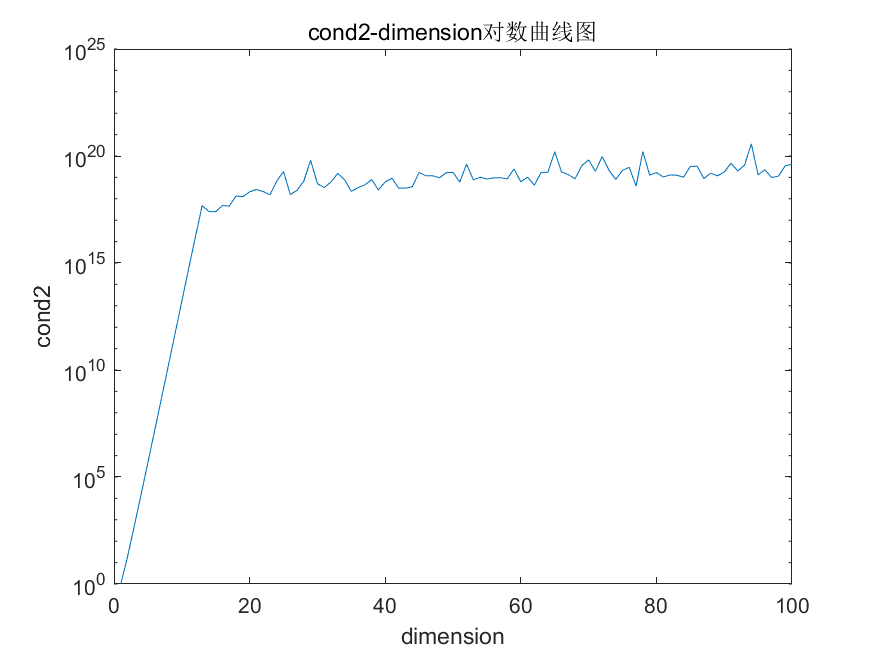
\includegraphics[width=0.8\textwidth]{../code/result/logcond2}
	\caption{\label{fig:1}使用cond()函数计算的2-条件数和矩阵阶数n在对数坐标下的曲线}
\end{figure}

\subsection{使用2-条件数的定义进行计算}
根据2-条件数的定义$cond_2(H)=||H||_2||H^{-1}||_2$,Matlab中有专门针对Hilbert矩阵逆矩阵的函数$invhilb()$,因此我们可以采用定义法来计算Hilbert矩阵的2-条件数。同样在对数坐标下,绘制出此种方法计算出的2-条件数和矩阵阶数的关系图如图\ref{fig:2}所示,从此图中可以看出,随着矩阵阶数的增加,对数化的2-条件数近似与阶数呈现线性关系,符合我们对Hilbert矩阵病态性的理解。

我们将对数化的2-条件数和矩阵阶数进行线性回归,得到拟合公式为: $cond2=10^{1.5257n-2.0758}$,相关系数$r\approx 1$,拟合之后图像如图\ref{fig:3}所示。

\begin{figure}[!h]
	\centering
	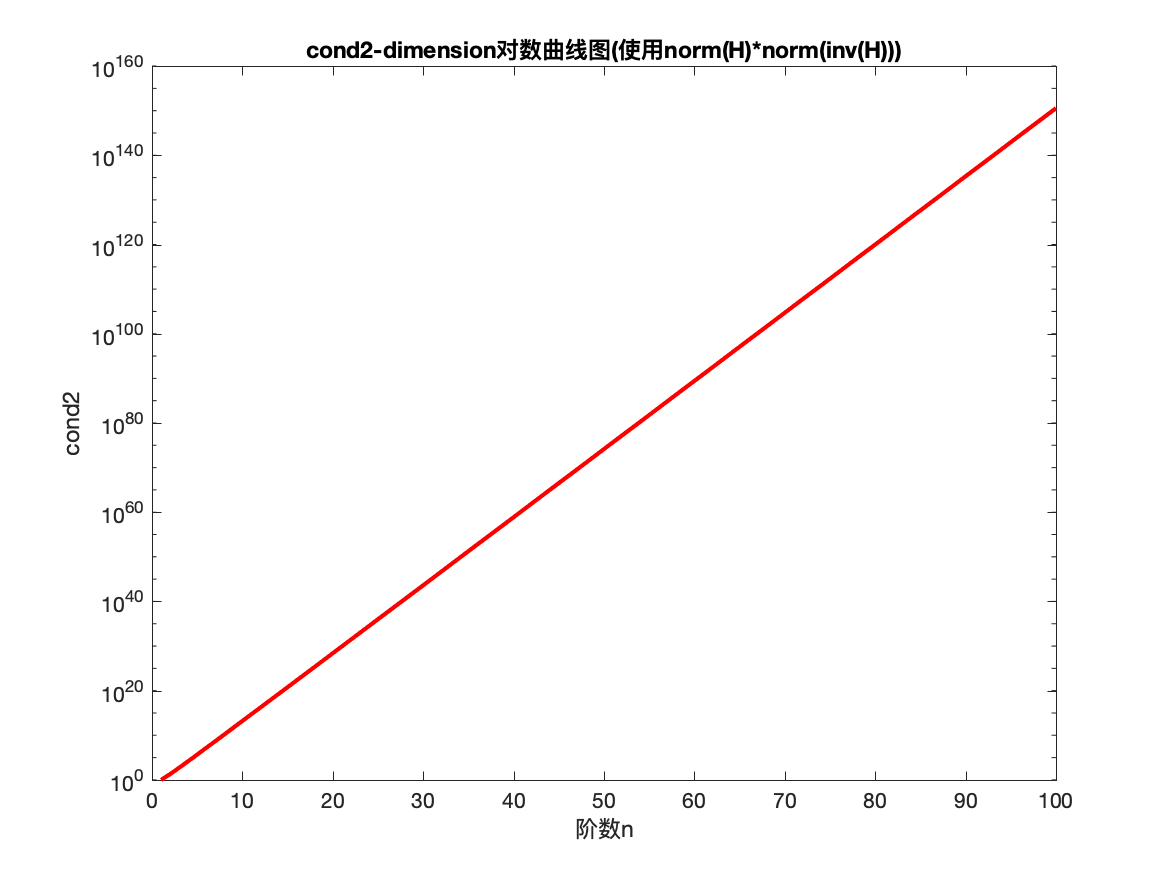
\includegraphics[width=0.8\textwidth]{../code/result/alogcond2}
	\caption{\label{fig:2}使用定义计算的2-条件数和矩阵阶数n在对数坐标下的曲线}
\end{figure}

\begin{figure}[!h]
	\centering
	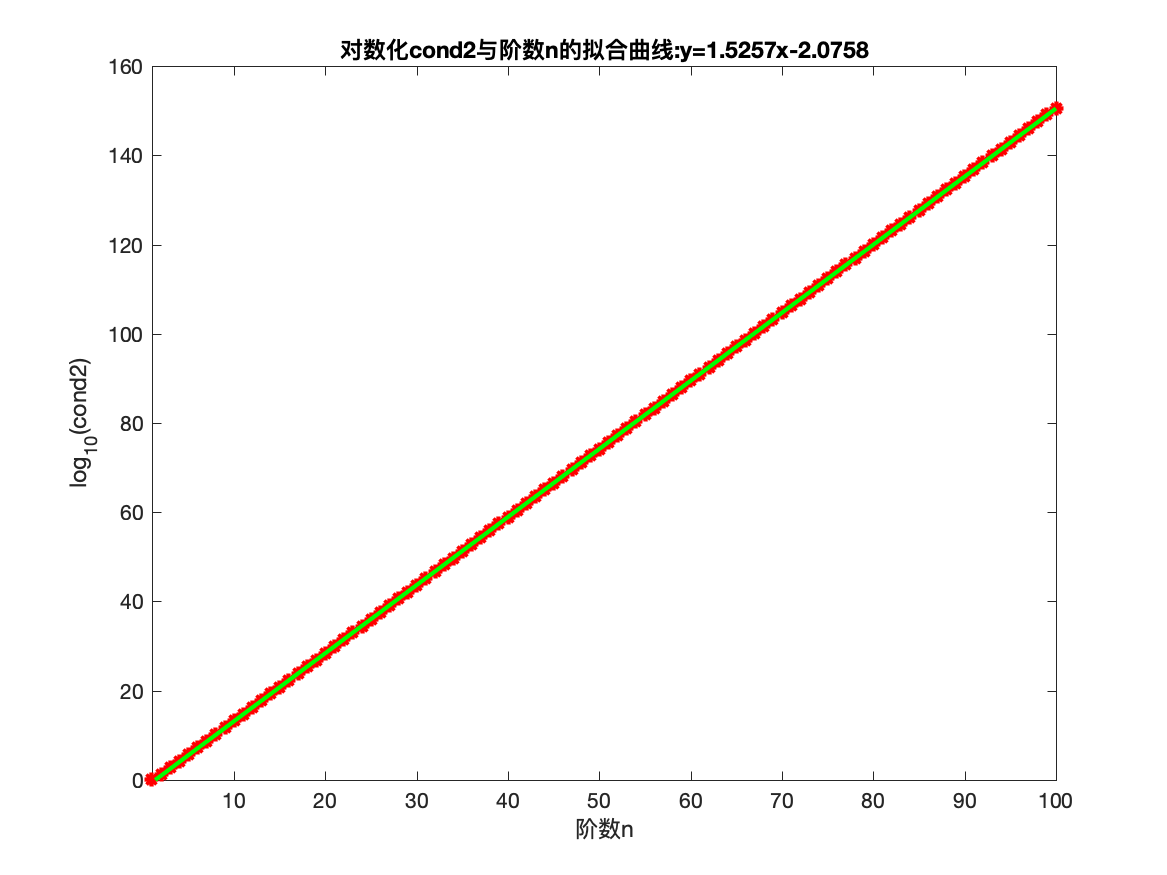
\includegraphics[width=0.8\textwidth]{../code/result/cond2fit}
	\caption{\label{fig:3}使用定义计算的2-条件数和矩阵阶数n在对数坐标下的曲线}
\end{figure}

\section{Gauss消去法}
用Gauss消去法将Hilbert矩阵消成上三角矩阵,然后求解结果。我们将阶数$n=2,5,10,20,50,100$的误差列表如表\ref{tab:table2}所示,从表中我们可以看出,随着矩阵阶数的增加,Gauss消去法的误差上升较快,当阶数为13时,误差就已经达到了3.0655,相对误差已经很大了,因此Gauss消去法不适和高阶Hilbert矩阵求解。我们绘制出$n=1\to100$时的Gauss消去法求解的相对误差曲线如图\ref{fig:4}所示。

\begin{table}[htbp]
	\centering
	\caption{Gauss消去法相对误差与阶数关系表格}
	\label{tab:table2}
	\begin{tabular}{|p{4cm}<{\centering}|p{6cm}<{\centering}|}
		\hline
		阶数n & Gauss消去法的相对误差 \\
		\hline
		2 & 5.66104886700368e-16 \\
		\hline
		5 & 1.55303820484067e-12 \\
		\hline
		10 & 0.000223773106799740 \\
		\hline
		20 & 23.5417423737487 \\
		\hline
		50 & 240.055736859534 \\
		\hline
		100 & 78.1201736046372 \\
		\hline
	\end{tabular}
\end{table}

\begin{figure}[!h]
	\centering
	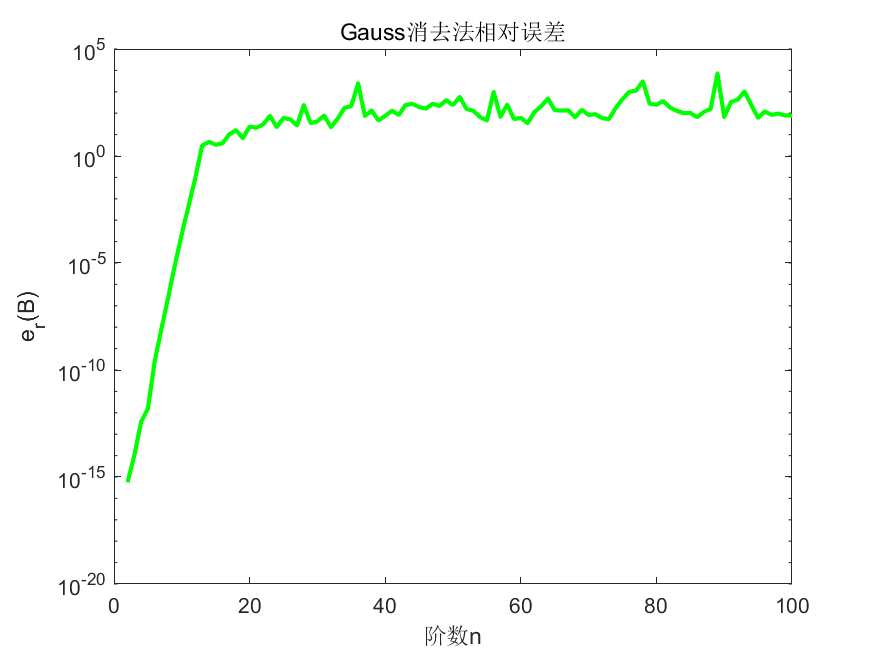
\includegraphics[width=0.8\textwidth]{../code/result/gausserror}
	\caption{\label{fig:4}Gauss消去法相对误差与阶数关系曲线图}
\end{figure}

\section{Jacobi矩阵迭代法}
设$H=D-L-U$,其中$D=diag(h_{11},h_{22},\cdots,h_{nn})$表示Hilbert矩阵$H$的对角线,$L$表示$H$的左下角元素的相反数,是一个下三角矩阵,$U$表示$H$的右上角元素的相反数,是一个上三角矩阵。因此,线性方程组$Hx=b$可以转换为$x=B_Jx+f$,其中$B_J=D^{-1}(L+U),f=D^{-1}b$,由此得到Jacobi迭代格式$x^{(k+1)}=B_Jx^{(k)}+f$。由于此种迭代格式只有当矩阵$B_J$的谱半径小于1时,迭代才是收敛的,因此,我们首先绘制出Jacobi迭代矩阵$B_J$的谱半径与阶数$n$的曲线图如图\ref{fig:5}所示,从图\subref{fig:b}中可以看出,当阶数$n>2$时,Jacobi迭代矩阵的谱半径就已经超过1了,因此当$n>2$时,Jacobi迭代法不收敛。当$n=2$时,我们设置当两次迭代的变化小于1e-6时,停止迭代,此时,Jicobi迭代相对误差为3.18555931744235e-07,误差比Gauss消去法在n=2时的误差还要大,因此,Jacobi迭代法不适合Hilbert矩阵线性方程组的求解。

\begin{figure}[!h] \centering 
	\subfigure[Jacobi迭代矩阵谱半径图] { \label{fig:a} 
		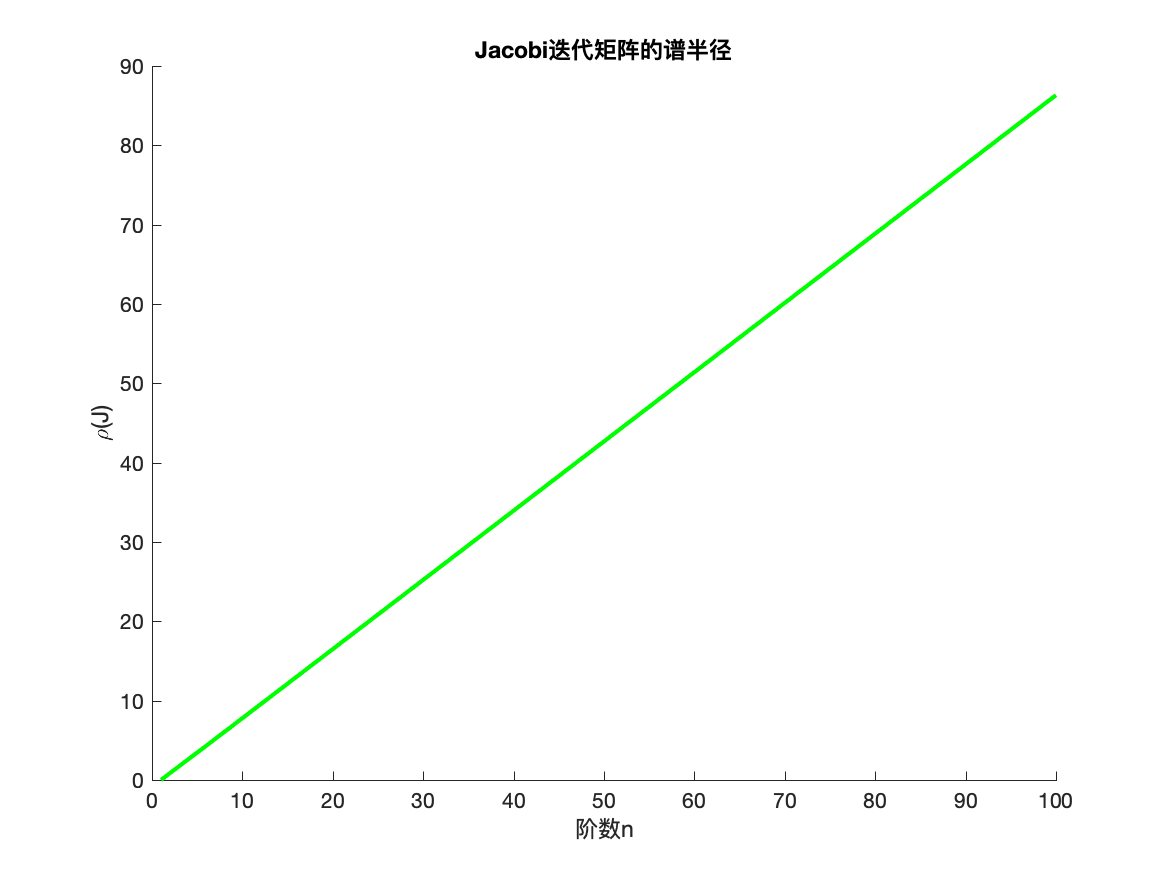
\includegraphics[width=0.48\columnwidth]{../code/result/jacobirho} 
	} 
	\subfigure[Jacobi迭代矩阵谱半径与1比较图] { \label{fig:b} 
		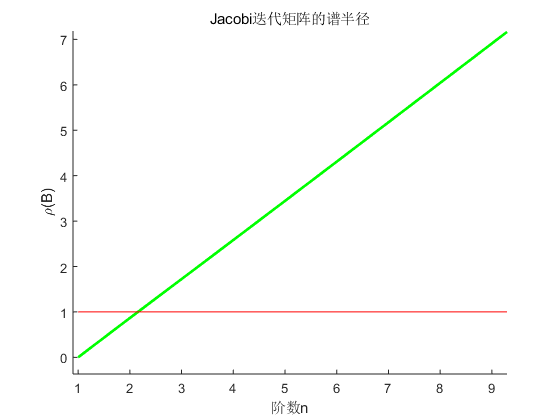
\includegraphics[width=0.48\columnwidth]{../code/result/jacobirho2} 
	} 
	\caption{Jacobi迭代矩阵谱半径图} 
	\label{fig:5} 
\end{figure}

\section{Gauss-Seidel矩阵迭代法}
设$H=D-L-U$,其中$D=diag(h_{11},h_{22},\cdots,h_{nn})$表示Hilbert矩阵$H$的对角线,$L$表示$H$的左下角元素的相反数,是一个下三角矩阵,$U$表示$H$的右上角元素的相反数,是一个上三角矩阵。因此,线性方程组$Hx=b$可以转换为$x=B_Gx+f$,其中$B_G=(D+L)^{-1}U,f=(D+L)^{-1}b$。与Jacobi矩阵迭代法类似,只有当矩阵$B_G$的谱半径小于1时,迭代才是收敛的,因此我们绘制出Gauss-Seidel迭代矩阵$B_G$的谱半径示意图如图\ref{fig:6}所示,从图中我们可以看出,当阶数$n\ge 13$时,谱半径已经$\ge 1$了,因此此时Gauss-Seidel迭代法已经不收敛了。由此可知,Gauss-Seidel迭代法效果比Jacobi迭代法支持的Hilbert矩阵阶数高一点,但是仍然不能够用于高阶Hilbert矩阵线性方程组的求解。

\begin{figure}[!h]
	\centering
	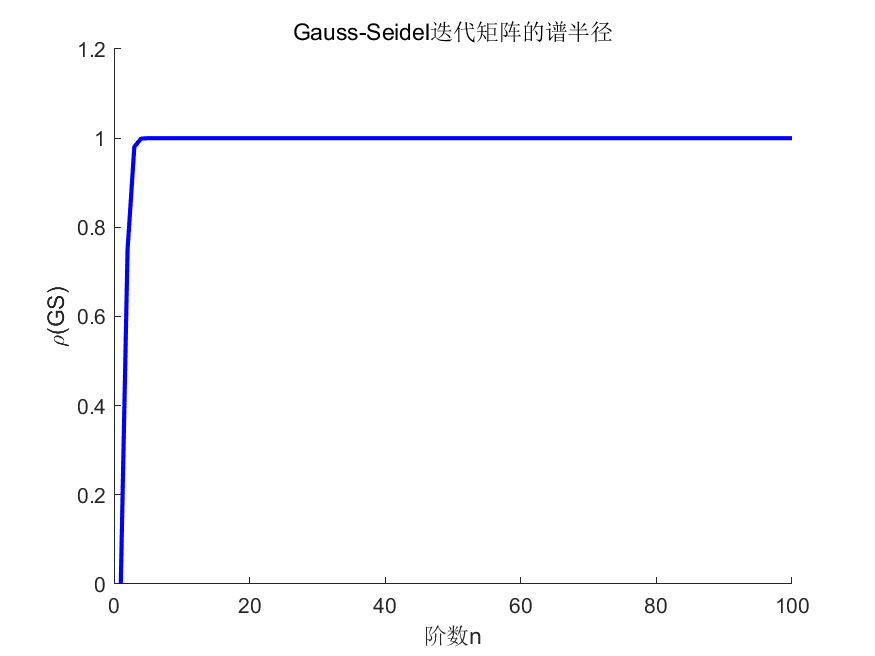
\includegraphics[width=0.8\textwidth]{../code/result/gsrho}
	\caption{\label{fig:6}Gauss-Seidel迭代矩阵谱半径与阶数n的关系图}
\end{figure}

\section{SOR迭代法}
设$H=D-L-U$,其中$D=diag(h_{11},h_{22},\cdots,h_{nn})$表示Hilbert矩阵$H$的对角线,$L$表示$H$的左下角元素的相反数,是一个下三角矩阵,$U$表示$H$的右上角元素的相反数,是一个上三角矩阵。因此,线性方程组$Hx=b$可以转换为$x=L_wx+f$,其中$L_w=(D-wL)^{-1}((1-w)D+wU),f=(D-wL)^{-1}b$。
\end{document}